Establishing correspondences across different object instances within the same category is a fundamental problem in computer vision~\cite{min2019spair71k,WahCUB_200_2011,yu2021AP10k,omninocs2024,zhang2023taleTwoFeatures,zhang2024tellingLeftFromRight,shi2021skeletonmerger,you2022ukpgan,ju2025robo_abc}. It underlies semantic matching, category-level reasoning, and downstream tasks such as object manipulation, image alignment, and visual understanding~\cite{zhang2023taleTwoFeatures,zhang2024tellingLeftFromRight,mariotti2024sphericalmap,Amoyal:CVPR:2026:GSA,Hirsch:NeurIPS:2025:FastJAM,Barel:ECCV:2024:SpaceJAM,wang2019visualcorrespondencerobotics,zhu2025densematcher,you2020,luo2023DiffusionHyperFeaturesTimeSpace,hedlin2023unsupervisedstablediffusion}. Compared to same-instance matching, cross-instance matching is substantially harder: objects may differ in geometry, proportions, local structure, texture, and appearance, while sharing only partially overlapping semantic parts. This paper focuses on semantic-geometric correspondences, where matches should preserve both semantic identity and geometric role when such distinctions are meaningful.

Progress in this direction is limited by the scarcity of scalable correspondence supervision. Existing datasets~\cite{min2019spair71k,cuttano2026marco,yu2021AP10k,zhu2025densematcher,WahCUB_200_2011,omninocs2024,you2020,lou2020human,pratikakis2016shrec_16,zuffi2017menagerie,groueix2018b3dcodeddataset,dyke2019shrec_19} rely heavily on manual annotation, which is costly, sparse, and difficult to scale across categories. AP-10K~\cite{yu2021AP10k} required 13 trained annotators, while Human Correspondence Consensus~\cite{lou2020humanCorrespondenceConsensus} uses 80 professional annotators and highlights the ambiguity of semantic point annotation. This ambiguity is inherent: across different instances, exact point-level correspondences are often not well-defined. We therefore ask whether approximate correspondences, if semantically meaningful, geometrically consistent, and sufficiently diverse, can provide effective supervision at scale.

We introduce SemGeo-Gen, an unsupervised pipeline for generating approximate cross-instance semantic-geometric correspondences from weakly aligned 3D object collections. Given rotation-aligned and scale-normalized rigid objects, SemGeo-Gen lifts multi-view DINOv2 features into 3D, uses them to assess semantic compatibility, aligns object instances with continuous piecewise-affine registration, and prunes geometrically plausible but semantically inconsistent matches. The resulting 3D correspondences can be projected into rendered views, yielding 3D--3D, 3D--2D, and 2D--2D supervision without manual annotation; see \autoref{fig:multi_modal_correspondences}. The construction also scales naturally with the number of available assets: a category with \(N\) objects yields up to \(\binom{N}{2}\) cross-instance pairs, and each accepted pair can generate dense 3D correspondences as well as many rendered 2D--2D training pairs.

We evaluate SemGeo-Gen in two complementary ways. First, we use the generated correspondences as synthetic pretraining data for recent semantic correspondence models and then fine-tune them on real SPair-71k annotations~\cite{min2019spair71k}, improving strong recent models without architectural modifications. Second, we compare our generated 3D correspondences to sparse human annotations from KeypointNet~\cite{you2020}, obtaining 92\% PCK@0.10, 97\% PCK@0.15, and 99\% PCK@0.20. These results indicate that automatically generated approximate correspondences, when constructed from 3D geometry and semantic features, can provide scalable supervision for cross-instance correspondence learning.

Our contributions are as follows:
\begin{enumerate}
    \item We introduce SemGeo-Gen, a fully automatic and unsupervised pipeline for generating dense approximate cross-instance semantic-geometric correspondences from weakly aligned 3D object collections, without point, part, or correspondence supervision.

    \item We combine lifted multi-view semantic features, deformable continuous piecewise-affine registration, and semantic correspondence pruning to generate matches constrained by both geometry and semantics.

    \item We project the generated 3D correspondences into rendered views, enabling combinatorially scalable 3D--3D, 3D--2D, and 2D--2D supervision for training image-based correspondence models.

    \item We show that the generated supervision improves recent semantic correspondence models on SPair-71k after real-data fine-tuning, yielding gains of up to 5 PCK points, while also agreeing well with sparse human KeypointNet annotations.
\end{enumerate}





\begin{figure}[t]
    \centering
    \begin{subfigure}[t]{0.33\linewidth}
        \centering
        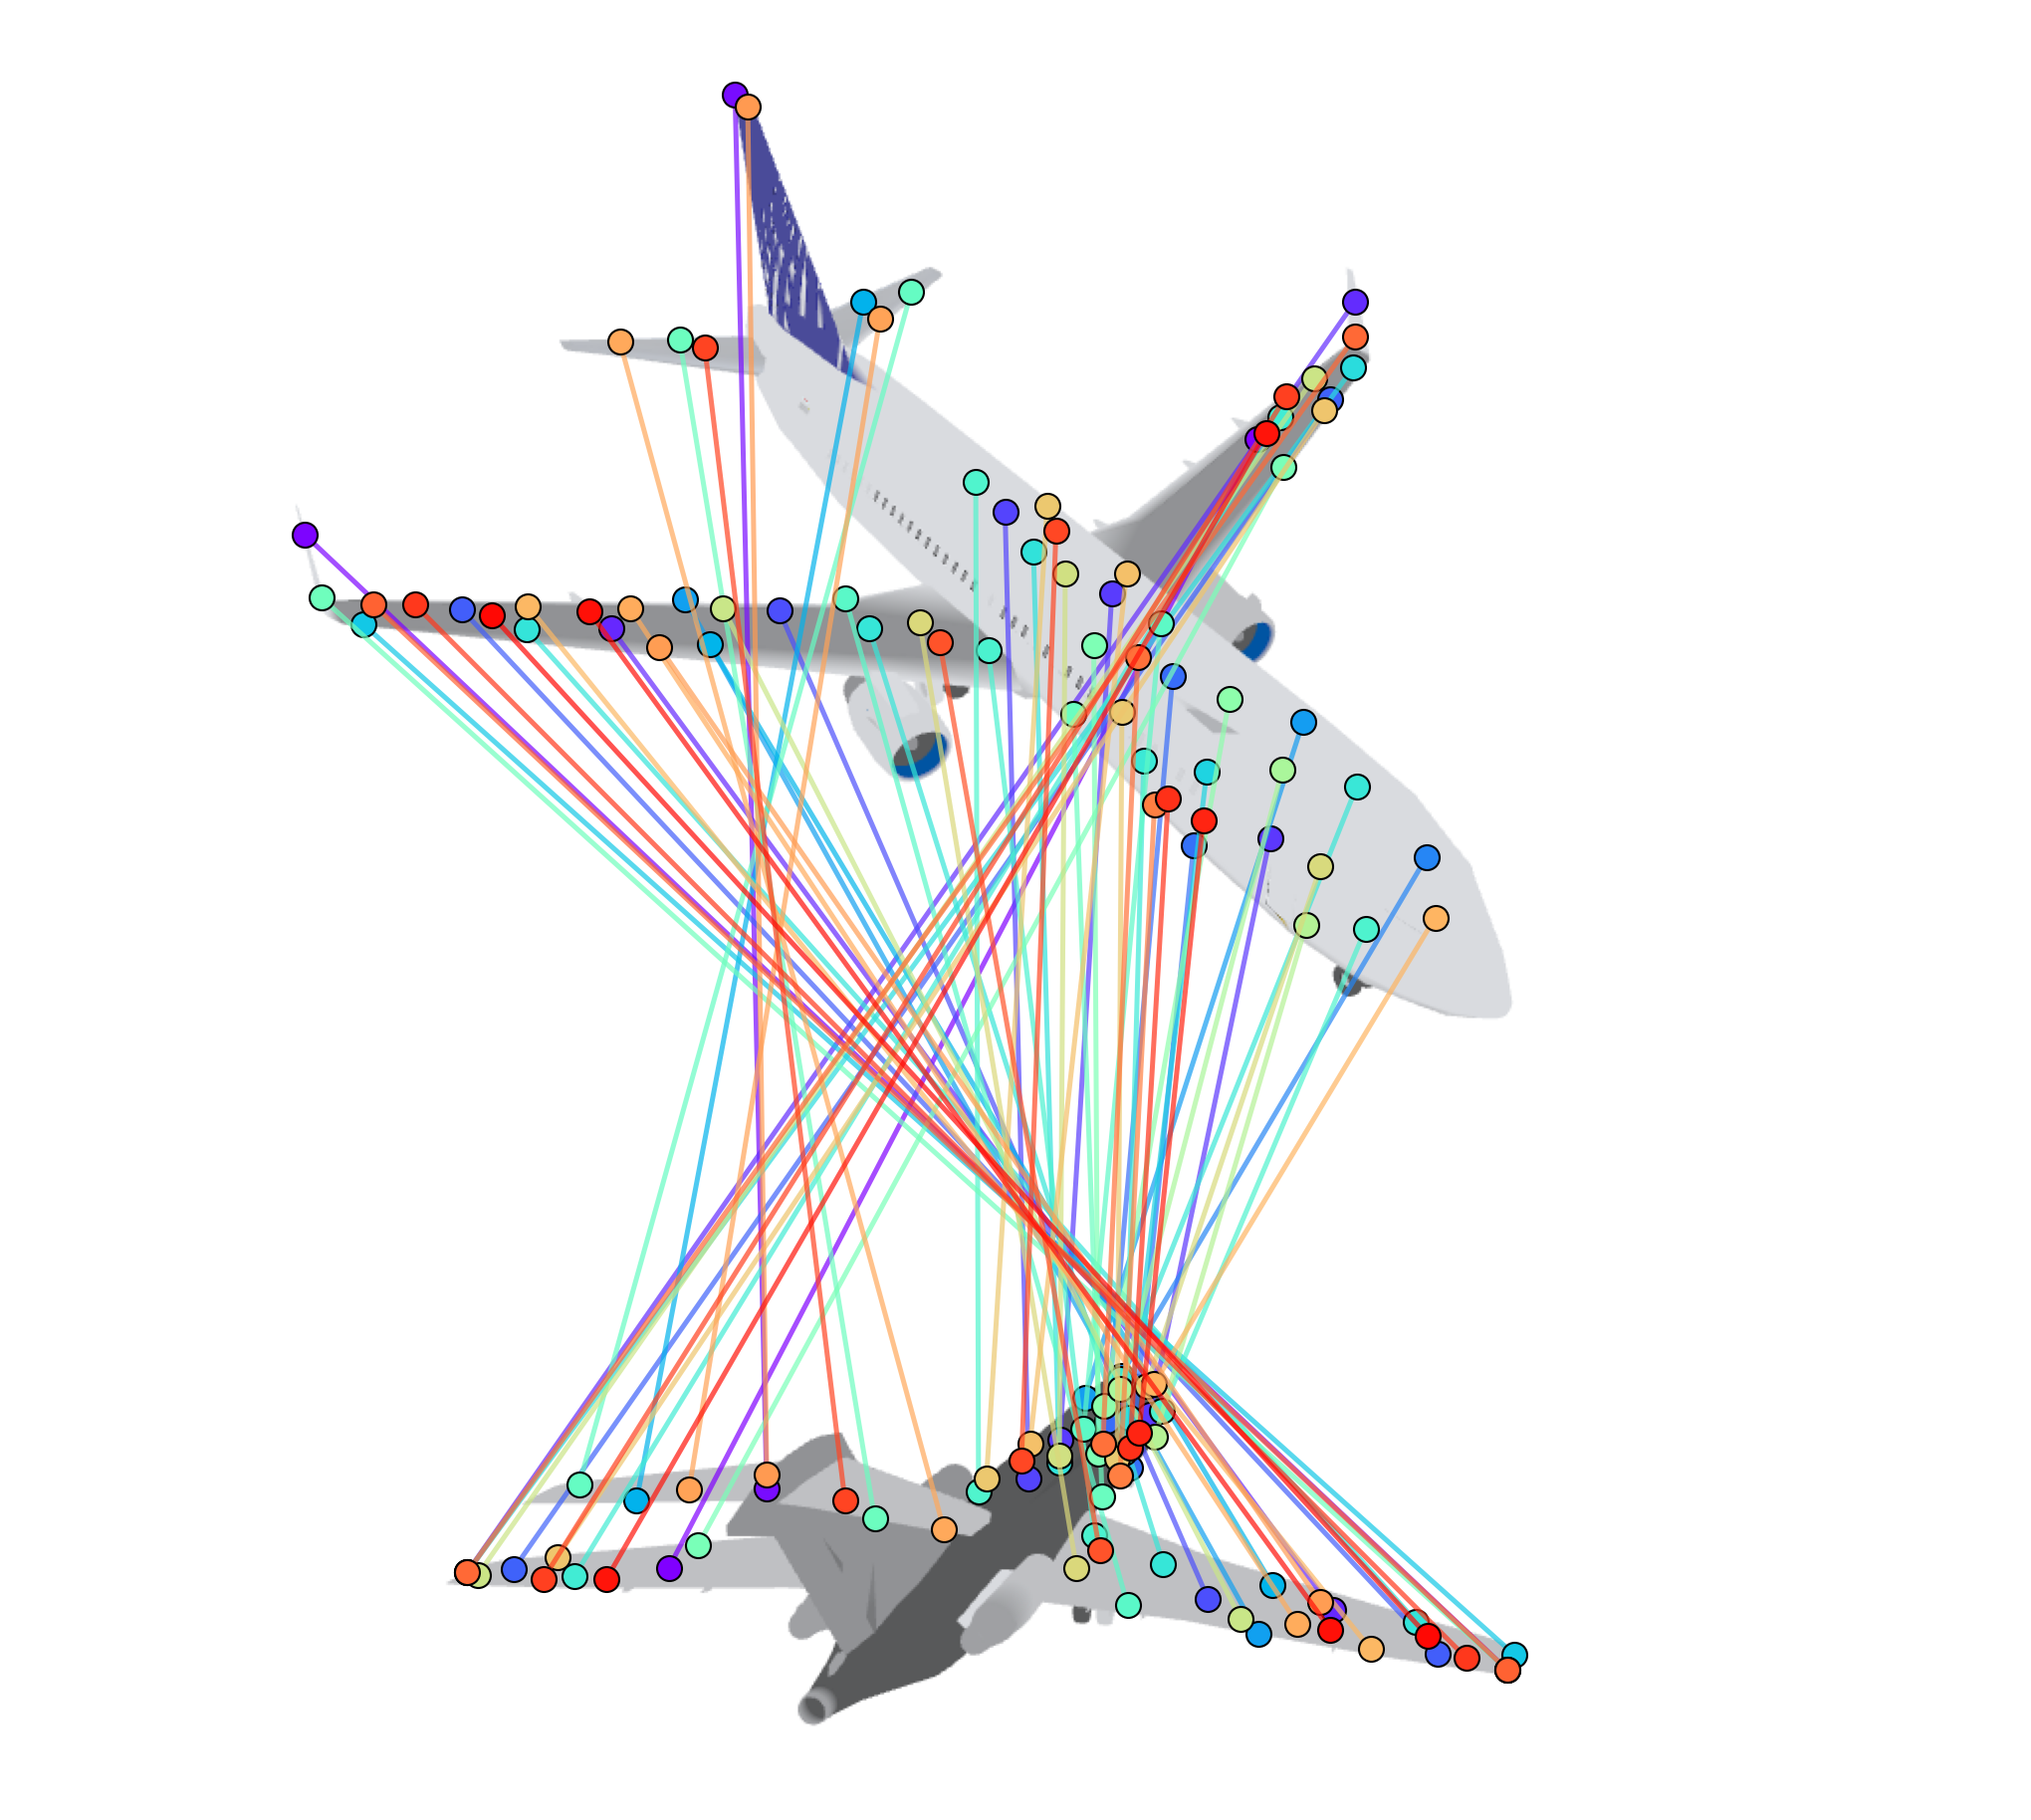
\includegraphics[
            width=\linewidth,
            trim={60pt 0pt 90pt 0pt},
            clip
        ]{figures/intro/2d_2d.png}
        \caption{2D--2D}
        \label{fig:corr_2d_2d}
    \end{subfigure}
    \begin{subfigure}[t]{0.30\linewidth}
        \centering
        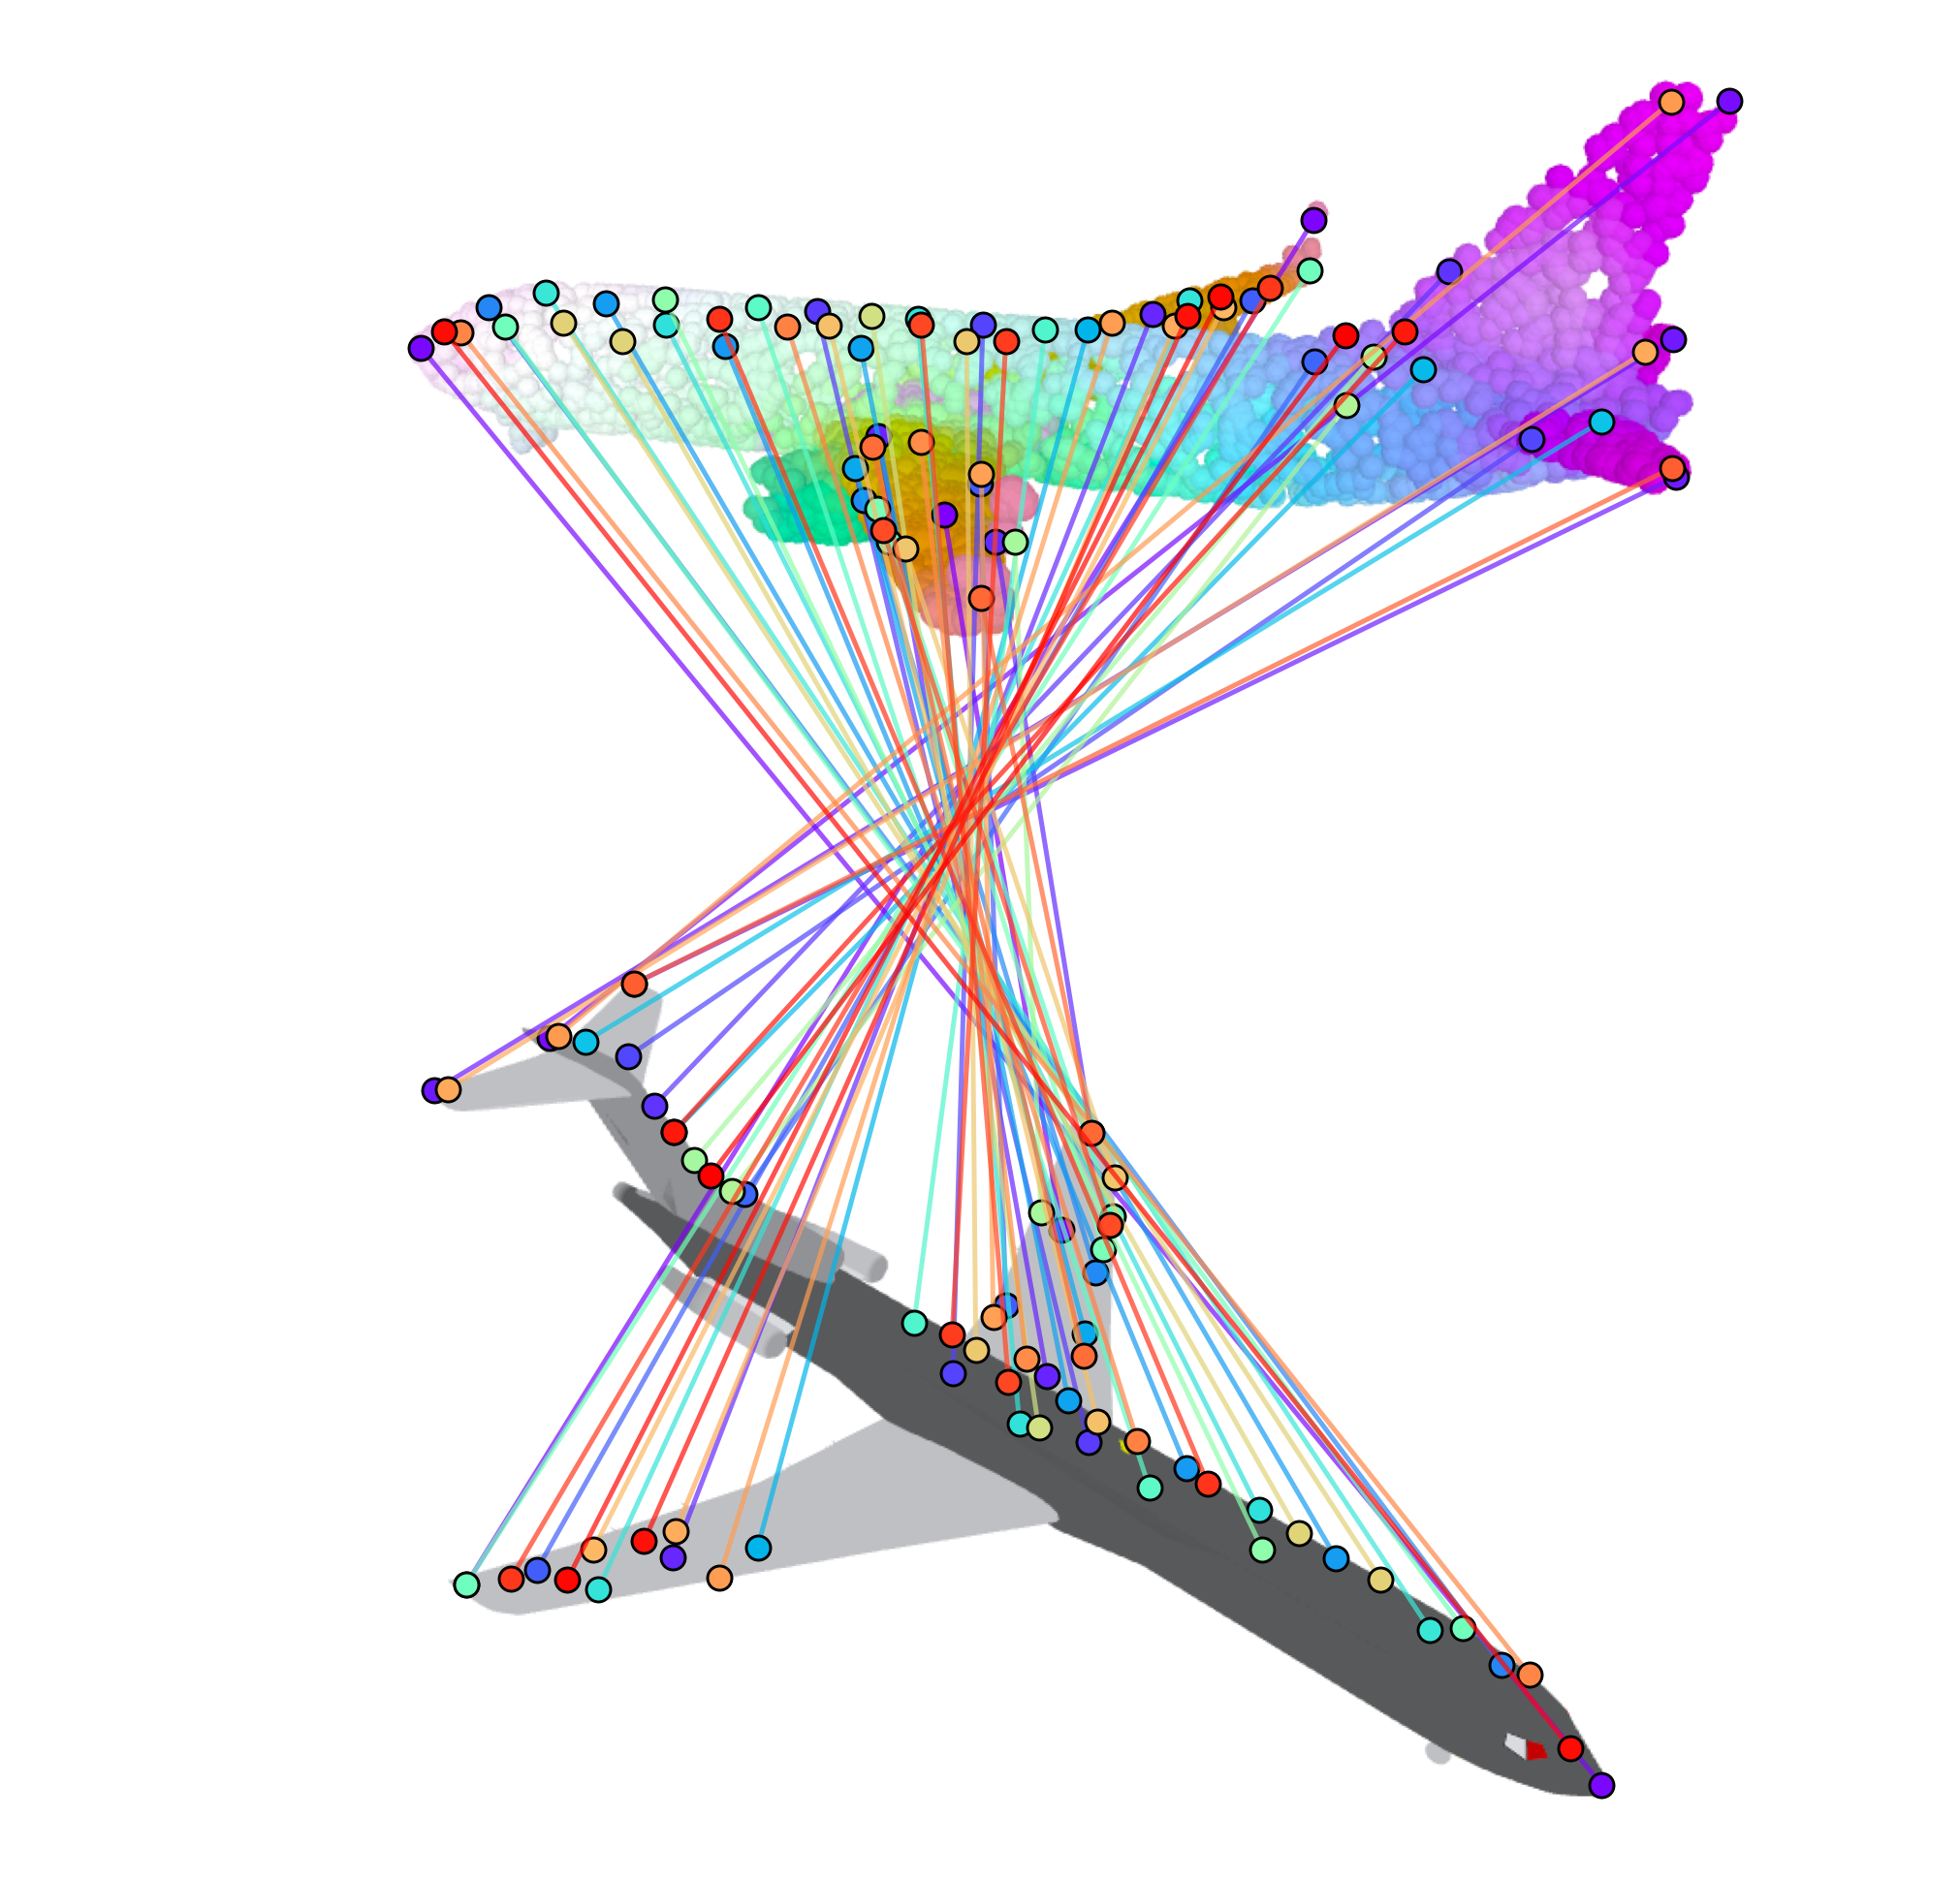
\includegraphics[
            width=\linewidth,
            trim={75pt 0pt 50pt 0pt},
            clip
        ]{figures/intro/3d_2d.png}
        \caption{3D--2D}
        \label{fig:corr_3d_2d}
    \end{subfigure}
    \begin{subfigure}[t]{0.33\linewidth}
        \centering
        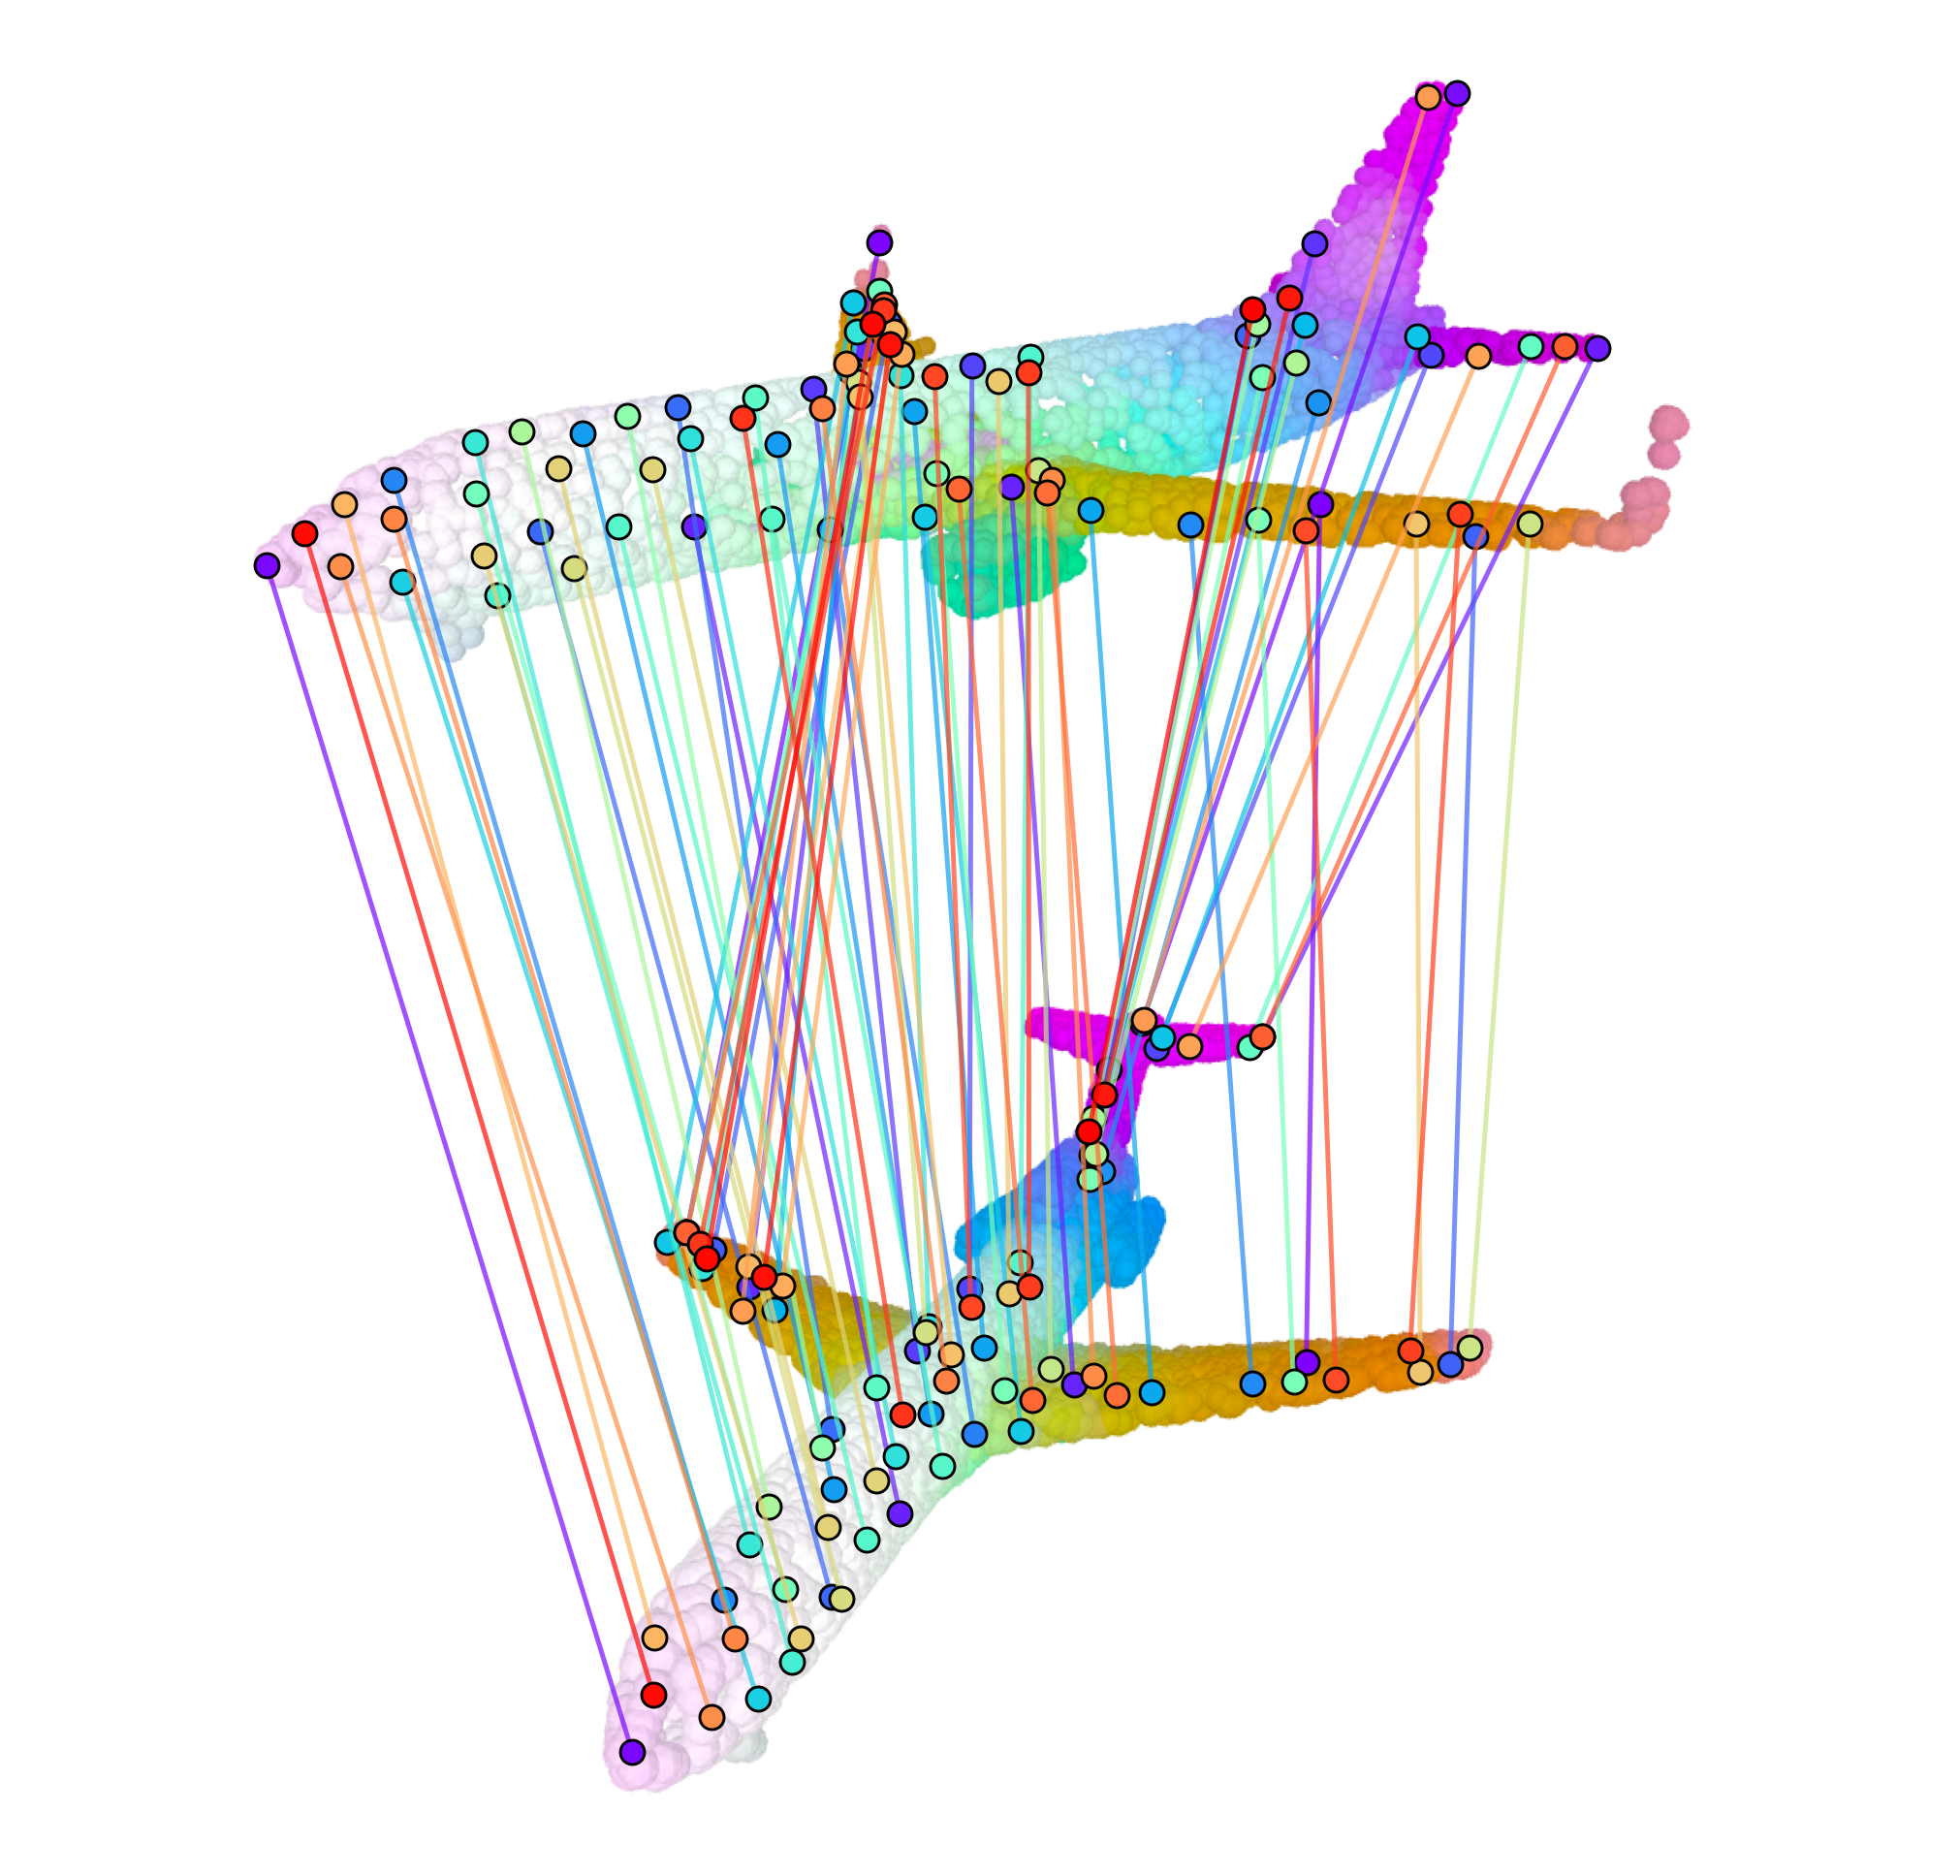
\includegraphics[
            width=\linewidth,
            trim={50pt 0pt 65pt 0pt},
            clip
        ]{figures/intro/3d_3d.png}
        \caption{3D--3D}
        \label{fig:corr_3d_3d}
    \end{subfigure}

     \caption{Approximate cross-instance semantic-geometric correspondences between two airplane instances across modalities. Left: 2D--2D correspondences between rendered views. Middle: 3D--2D correspondences between a 3D object and a rendered view. Right: 3D--3D correspondences between object surfaces. Colors in 3D visualize the lifted DINOv2 features reduced to three dimensions.}
    \label{fig:multi_modal_correspondences}
\end{figure}
